\documentclass{lab}

\usepackage[utf8]{inputenc}
\usepackage{graphicx}
\usepackage{tocloft}
\usepackage{amssymb}
\usepackage{xcolor}
\usepackage{enumitem}
\usepackage{amsmath} 
\usepackage{animate}
\usepackage{graphicx}
\usepackage[T1]{fontenc} 
\usepackage[top=0.5in, bottom=0.5in, left=0.5in, right=0.5in]{geometry}
\usepackage{mathrsfs}
\usepackage{hyperref}
\usepackage{wrapfig}
\usepackage{indentfirst}
\usepackage{mathtools}
\usepackage[export]{adjustbox}
\usepackage{scrextend}
\usepackage{animate}
\usepackage{float}
\newcommand\tab[1][1cm]{\hspace*{#1}}
\geometry{
    margin=0.5in,
    left=2.2cm,
    right=2.2cm,
    headheight=17pt,
    headsep=1cm, % Increase the margin from the top for the header
    includehead,
    includefoot
}

% python color
\usepackage{listings}
\usepackage{xcolor}
\usepackage{caption}

% Define VSC Dark+ colors
\definecolor{vscode-background}{rgb}{0.0, 0.0, 0.0}
\definecolor{vscode-foreground}{rgb}{0.96, 0.96, 0.96}
\definecolor{vscode-comment}{rgb}{0.51, 0.51, 0.51}
\definecolor{vscode-orange}{rgb}{1.0, 0.6, 0.0}
\definecolor{vscode-yellow}{rgb}{0.98, 0.83, 0.26}
\definecolor{vscode-green}{rgb}{0.19, 0.8, 0.35}
\definecolor{vscode-cyan}{rgb}{0.16, 0.71, 0.73}
\definecolor{vscode-blue}{rgb}{0.13, 0.48, 0.78}
\definecolor{vscode-purple}{rgb}{0.58, 0.4, 0.72}
\definecolor{vscode-pink}{rgb}{0.8, 0.36, 0.36}

% Define the style
\lstdefinestyle{vscode-darkplus-python}{
    language=Python,
    backgroundcolor=\color{vscode-background},
    basicstyle=\color{vscode-foreground}\ttfamily\small,
    commentstyle=\color{vscode-comment},
    keywordstyle=\color{vscode-orange},
    numberstyle=\tiny\color{vscode-comment},
    numbers=left,
    stringstyle=\color{vscode-green},
    emphstyle=\color{vscode-pink},
    frame=none,
}
% Change the caption label to "Kod źródłowy"
\DeclareCaptionLabelFormat{myformat}{Kod źródłowy #2}

\usepackage[T1]{fontenc}
\usepackage[polish]{babel}
\usepackage[utf8]{inputenc}
\usepackage{amsmath}
\usepackage{listings}
\usepackage{hyperref}
\usepackage{pythonhighlight}
\usepackage{amssymb}
\usepackage{mathtools}
\usepackage{array}
\usepackage{xpatch}

\xpretocmd{\part}{\setcounter{section}{0}}{}{}
\usepackage[margin=0.5in,
    left=2.2cm,
    right=2.2cm,
    headheight=17pt,
    includehead, includefoot]{geometry}
    
%% nagłówek
\usepackage{fancyhdr}
\usepackage{tikz}
\usepackage{pgfplots}
\usepackage{pgfplotstable}
\pagestyle{fancy}
\fancyhf{}
\rhead{Rachunek Prawdopodobieństwa i Statystyka}
\lhead{Porównanie Algorytmów Minimalizacji Stochastycznej}
\rfoot{\thepage}

%% Podmiana \part na obecne wyświetlanie
\makeatletter
\renewcommand\@part[2][]{%
  \ifnum \c@secnumdepth >-2\relax
    \refstepcounter{part}%
    \addcontentsline{toc}{part}{\thepart#2}%
  \else
    \addcontentsline{toc}{part}{#2}%
  \fi
  \markboth{}{}%
  {\raggedright % Align title to the left
   \interlinepenalty \@M
   \normalfont
   \ifnum \c@secnumdepth >-2\relax
     \Large\bfseries \thepart\hspace{1em}%
   \fi
   \huge \bfseries #2\par}%
  \@endpart
}
\makeatother

\renewcommand\thepart{\Roman{part}. }

\addtokomafont{labelinglabel}{\sffamily}

\renewcommand{\cftsecleader}{\cftdotfill{\cftdotsep}}
\renewcommand{\cftsubsecleader}{\cftdotfill{\cftdotsep}}


\begin{document}
\captionsetup[lstlisting]{labelformat=myformat}

\begin{figure*}
    \centering
    
\includegraphics{img/agh.png}
\end{figure*}
\title{\Huge \textbf{Porównanie Algorytmów Minimalizacji Stochastycznej}\\ Pure-Random-Search i Multi-Start}
\author{Radosław Rolka, Mateusz Kochelski\\Rachunek Prawdopodobieństwa i Statystyka\\Informatyka WI AGH, II rok}
\date{styczeń 2023}

\maketitle
\newpage
\tableofcontents
\thispagestyle{fancy} 
\newpage

\part{Wstęp}
\section{Wybrane Algorytmy Minimalizacji}
\subsection{Pure-Random-Search}
Losujemy po kolei zadaną z góry liczbę punktów z rozkładem jednostajnym w zadanej dziedzinie. Każdy wylosowany punkt porównujemy z aktualnie zapamiętanym minimum i jeśli wartość minimalizowanej funkcji w tym punkcie jest mniejsza, to ten punkt zapamiętujemy jako aktualny punkt minimalny. Wartość funkcji w ostatnim zapamiętanym punkcie stanowi wynik algorytmu.

\subsection{Multi-Start}
Losujemy (podobnie jak poprzednio) zadaną liczbę punktów z rozkładem jednostajnym w dziedzinie przeszukiwania, a następnie z każdego z wylosowanych punktów startujemy numeryczną metodę optymalizacji lokalnej, z wykorzystaniem metody L-BFGS-B. Wynikiem algorytmu jest wartość optymalizowanej funkcji w tym z punktów zwróconych przez uruchomienia metody lokalnej, w którym ta wartość jest najmniejsza.

\section{Wybrane Funkcje}
\subsection{Alpine01}
Alpine01 jest funkcją wielowymiarową, która dla $n$ wymiarowego wektora $x = (x_1, ... , x_n) \in \[−10; 10\]^n$ zwraca wartość:
\begin{equation*}
    f(x) = \sum_{i=1}^{n} | x_i*sin(x_i) + 0.1*x_i |
\end{equation*}
\begin{figure}[H]
  \centering
  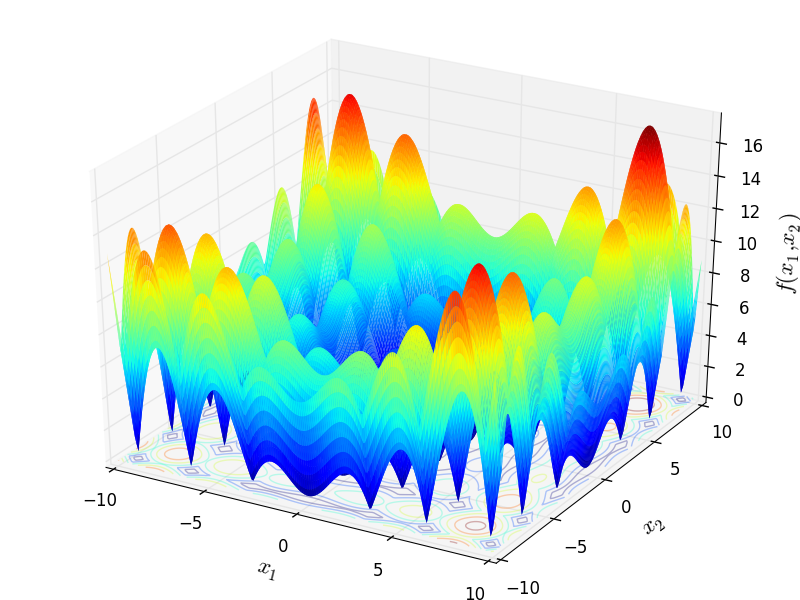
\includegraphics[width=0.7\textwidth]{img/Alpine01.png}
  \caption{Wykres funkcji Alpine01 dla 2 wymiarów.}
\end{figure}

\subsection{funkcja Ackley’a}
Funkcja Ackley'a jest funkcją wielowymiarową, która dla $n$ wymiarowego wektora $x = (x_1, ... , x_n)$ zwraca wartość:
\begin{equation*}
    f(x) = -20e^{-0.2\sqrt{\frac{1}{n}\sum_{i=1}^{n} x^2_i}} - e^{\frac{1}{n}\sum_{i=1}^{n}cos(2\pi x_i)} + 20 + e
\end{equation*}
\begin{figure}[H]
  \centering
  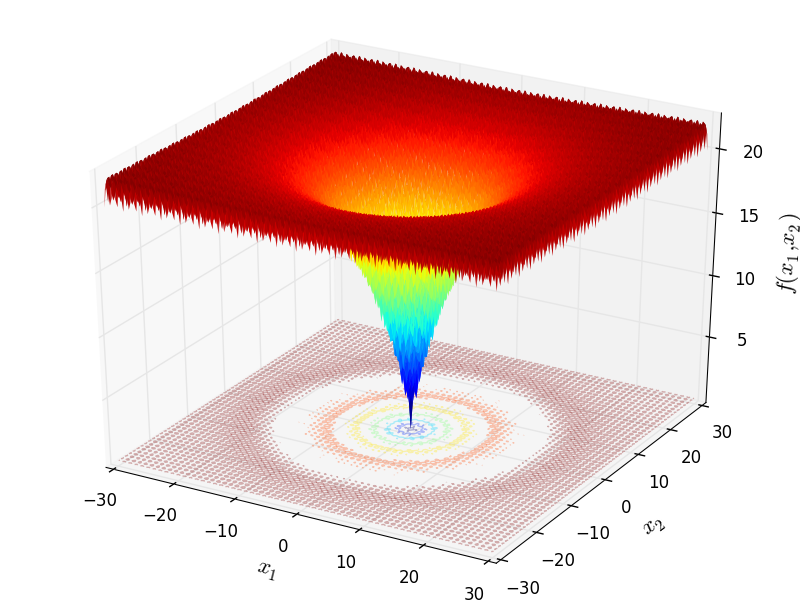
\includegraphics[width=0.7\textwidth]{img/Ackley.png}
  \caption{Wykres funkcji Ackley'a dla 2 wymiarów.}
\end{figure}

\newpage
\part{Metodologia}
\section{Sposób wykonania}
Porównania zostały wykonane dla obu metod w przypadkach, gdy liczba wymiarów wynosiła:
\begin{itemize}
    \item $dim = 2$
    \item $dim = 10$
    \item $dim = 20$
\end{itemize}
\par Dla każdego przypadku metoda została wykonana 50 razy. Ze względu na wielokrotne uruchamianie MS, wynikające z obliczania gradientu, Koszt wykonania będzie wyższy niż PRS. Aby zachować zrównoważony budżet wykorzystamy średni koszt MS wszystkich startów i proporcjonalnie zwiększymy koszt PRS.
\newline\par
Analizę statystycznej istotności różnicy między średnimi wynikami algorytmów dokonujemy poprzez test t Studenta dla dwóch prób. Robimy tak ze względu na dużą ilość prób, przez co możemy zakładać że rozkład średniej jest rozkładem normalnym.

\section{Kod źródłowy}
\subsection{Pure-Random-Search}
\begin{lstlisting}[
  style=vscode-darkplus-python,
  caption={Funkcja wykorzystująca metodę PRS.},
  label=lst:python_code,
  captionpos=b
]
PRS = function(func,dim,random_trials) {
  f = func(dim)
  result = Inf
  RandomPoints = replicate(random_trials,
                           runif(dim, 
                                 getLowerBoxConstraints(f), 
                                 getUpperBoxConstraints(f)))
  for(i in 1:random_trials) {
    result=min(result,f(RandomPoints[,i]))
  }
  return (result)
}
\end{lstlisting}

\subsection{Multi-Start}
\begin{lstlisting}[
  style=vscode-darkplus-python,
  caption={Funkcja wykorzystująca metodę MS.},
  label=lst:python_code,
  captionpos=b
]
MS_Minimalize <- function(func, dim, points_quantity) {
  f <- func(dim)
  values <- c(1:points_quantity)
  counter <- c(1:points_quantity) 
  MS <- replicate(n = points_quantity, optim(runif(dim, 
                                                   getLowerBoxConstraints(f), 
                                                   getUpperBoxConstraints(f)), 
                                             f, 
                                             method = "L-BFGS-B",
                                             lower = getLowerBoxConstraints(f), 
                                             upper = getUpperBoxConstraints(f))
  )
  for (i in 1:points_quantity) {
    values[i]  = MS[[2, i]]
    counter[i] = MS[[3, i]][2] 
  }
  return (list(min(values), mean(counter)))
}
\end{lstlisting}

\subsection{Porównanie metod}
\begin{lstlisting}[
  style=vscode-darkplus-python,
  caption={Funkcja wykorzystująca t-testy.},
  label=lst:python_code,
  captionpos=b
]
compare_MS_to_PRS = function(dim,func,numberOfRuns,NumberOfPoints) {
  MS_resultsCounter = replicate(numberOfRuns,MS_Minimalize(func,dim,NumberOfPoints))
  MS_Counter = mean(as.numeric(MS_resultsCounter[2,]))
  MS_results = as.numeric(MS_resultsCounter[1,])
  PRS_results = replicate(numberOfRuns,PRS(func,dim,NumberOfPoints*MS_Counter))
  print(t.test(MS_results,PRS_results,conf.level=0.95))
}
\end{lstlisting}

\newpage
\part{Porównanie}
\section{dim = 2}
\subsection{Wykresy Alpine01}
\subsubsection{Pure-Random-Search}
\begin{figure}[H]
  \centering
  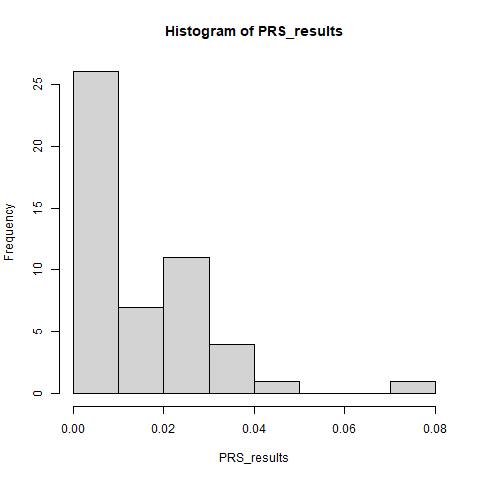
\includegraphics[width=0.7\textwidth]{img/dim2_PRS_Alpine01_his.png}
  \caption{Histogram funkcji Alpine01, metody PRS, dla 2 wymiarów.}
\end{figure}
\begin{figure}[H]
  \centering
  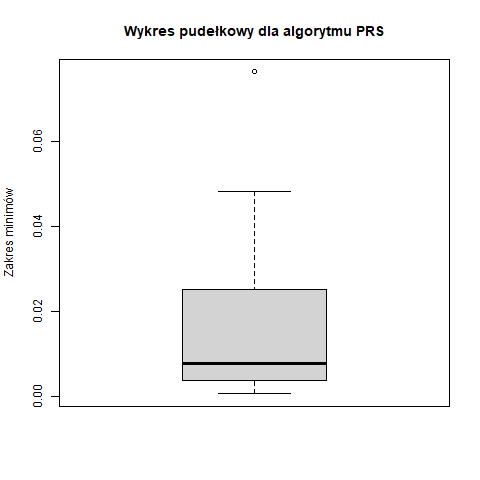
\includegraphics[width=0.56\textwidth]{img/dim2_PRS_Alpine01.png}
  \caption{Wykres pudełkowy funkcji Alpine01, metody PRS, dla 2 wymiarów.}
\end{figure}

\subsubsection{Multi-Start}
\begin{figure}[H]
  \centering
  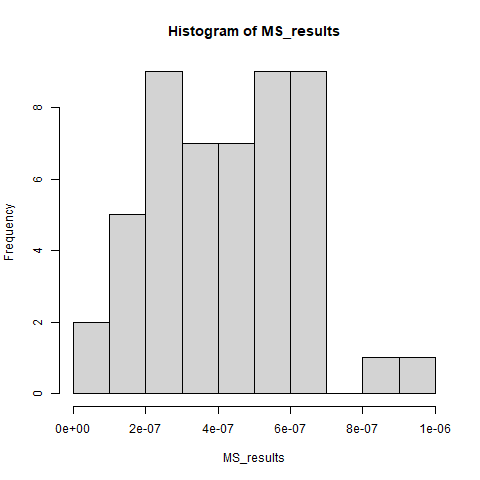
\includegraphics[width=0.56\textwidth]{img/dim2_MS_Alpine01_his.png}
  \caption{Histogram funkcji Alpine01, metody MS, dla 2 wymiarów.}
\end{figure}
\begin{figure}[H]
  \centering
  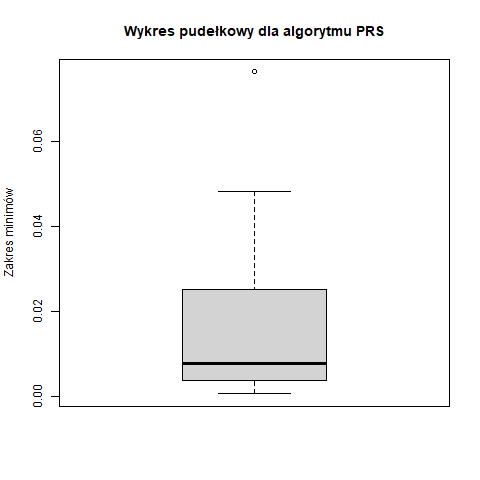
\includegraphics[width=0.7\textwidth]{img/dim2_MS_Alpine01.png}
  \caption{Wykres pudełkowy funkcji Alpine01, metody MS, dla 2 wymiarów.}
\end{figure}

\subsubsection{Obserwacje}
 \begin{figure}[H]
     \centering
     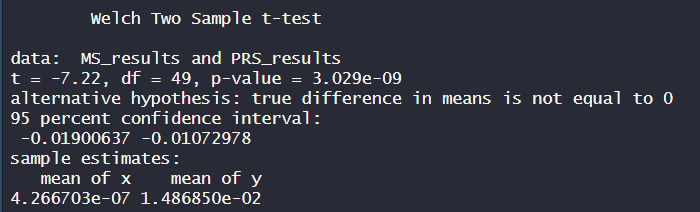
\includegraphics[width=0.9\linewidth]{img/T1.png}
     \caption{Wynik funkcji t.test.}
     \label{fig:enter-label}
 \end{figure}

Średnia wyników dla metody PRS wynosi $1.486850*10^{-2}$, natomiast dla metody MS wynosi $4.266703*10^{-7}$. Jest to różnica 5 rzędów wielkości na korzyść metody MS. P-value wynosi $3.029*10^{-9}$, a przedział ufności nie zawiera zera. Z tego wynika że odrzucamy hipotezę zerową, czyli średnie wyników obu algorytmów nie są sobie równe.

\subsection{Wykresy funkcji Ackley’a}
\subsubsection{Pure-Random-Search}
\begin{figure}[H]
  \centering
  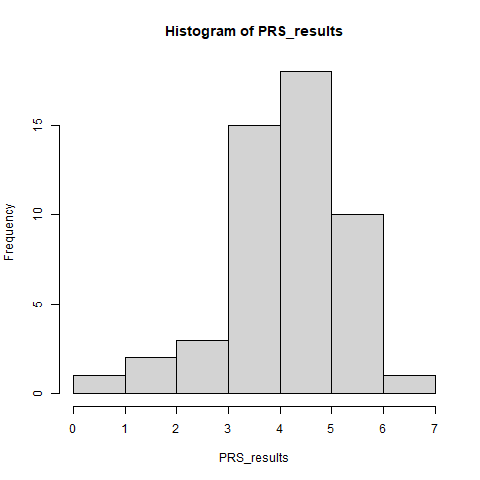
\includegraphics[width=0.7\textwidth]{img/dim2_PRS_Ackley_his.png}
  \caption{Histogram funkcji Ackley'a, metody PRS, dla 2 wymiarów.}
\end{figure}
\begin{figure}[H]
  \centering
  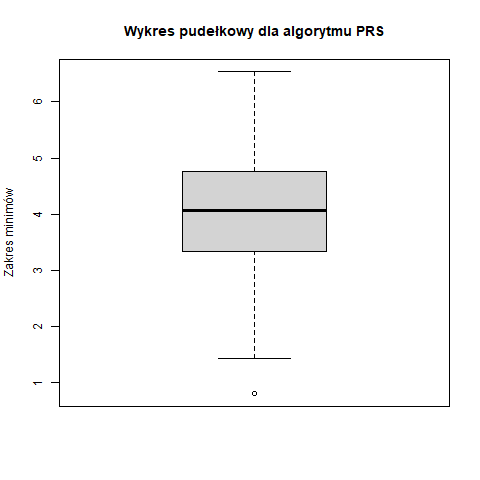
\includegraphics[width=0.56\textwidth]{img/dim2_PRS_Ackley.png}
  \caption{Wykres pudełkowy funkcji Ackley'a, metody PRS, dla 2 wymiarów.}
\end{figure}

\subsubsection{Multi-Start}
\begin{figure}[H]
  \centering
  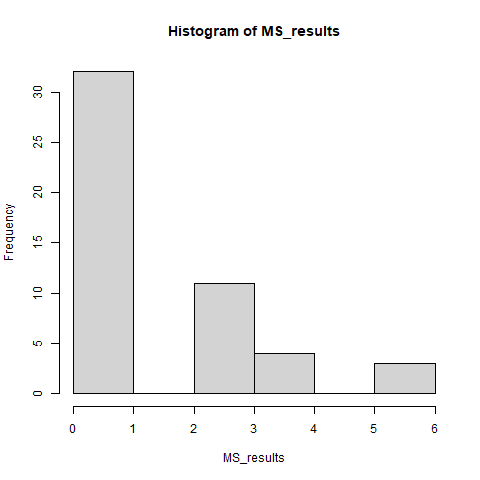
\includegraphics[width=0.56\textwidth]{img/dim2_MS_Ackley_his.png}
  \caption{Histogram funkcji Ackley'a, metody MS, dla 2 wymiarów.}
\end{figure}
\begin{figure}[H]
  \centering
  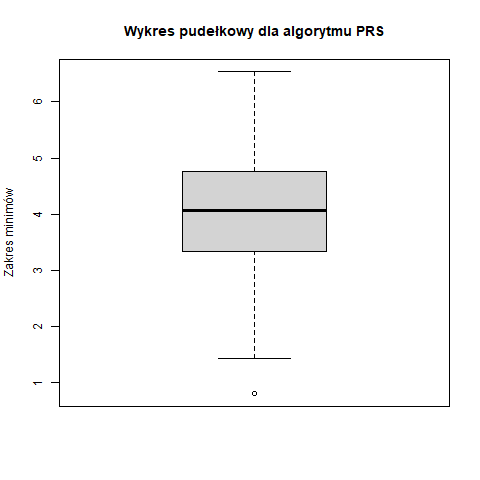
\includegraphics[width=0.7\textwidth]{img/dim2_MS_Ackley.png}
  \caption{Wykres pudełkowy funkcji Ackley'a, metody MS, dla 2 wymiarów.}
\end{figure}

\subsubsection{Obserwacje}
 \begin{figure}[H]
     \centering
     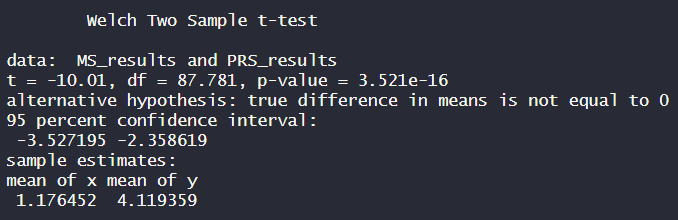
\includegraphics[width=0.9\linewidth]{img/T2.png}
     \caption{Wynik funkcji t.test.}
     \label{fig:enter-label}
 \end{figure}

 Średnia wyników dla metody PRS wynosi $4.119359$, natomiast dla metody MS wynosi $1.176452$. Metoda MS jest dokładniejsza. P-value wynosi $3.521*10^{-16}$, a przedział ufności nie zawiera zera. Z tego wynika że odrzucamy hipotezę zerową, czyli średnie wyników obu algorytmów nie są sobie równe.

\section{dim = 10}
\subsection{Wykresy Alpine01}
\subsubsection{Pure-Random-Search}
\begin{figure}[H]
  \centering
  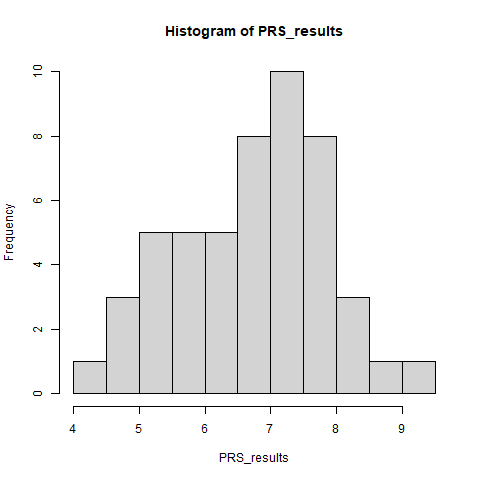
\includegraphics[width=0.7\textwidth]{img/dim10_PRS_Alpine01_his.png}
  \caption{Histogram funkcji Alpine01, metody PRS, dla 10 wymiarów.}
\end{figure}
\begin{figure}[H]
  \centering
  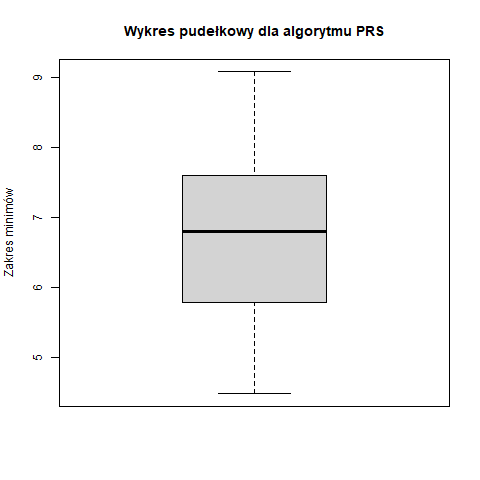
\includegraphics[width=0.56\textwidth]{img/dim10_PRS_Alpine01.png}
  \caption{Wykres pudełkowy funkcji Alpine01, metody PRS, dla 10 wymiarów.}
\end{figure}

\subsubsection{Multi-Start}
\begin{figure}[H]
  \centering
  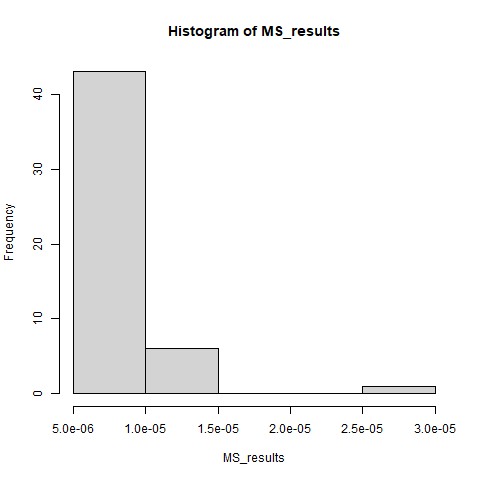
\includegraphics[width=0.56\textwidth]{img/dim10_MS_Alpine01_his.png}
  \caption{Histogram funkcji Alpine01, metody MS, dla 10 wymiarów.}
\end{figure}
\begin{figure}[H]
  \centering
  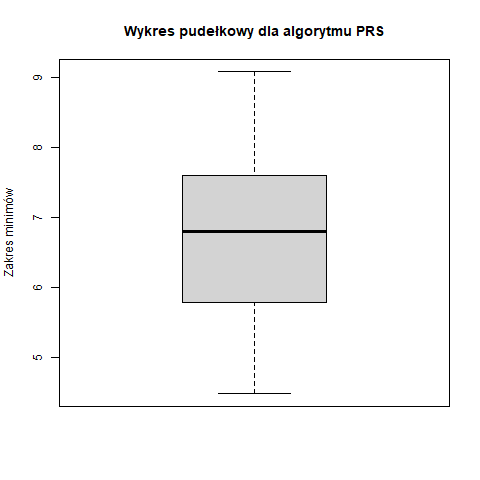
\includegraphics[width=0.7\textwidth]{img/dim10_MS_Alpine01.png}
  \caption{Wykres pudełkowy funkcji Alpine01, metody MS, dla 10 wymiarów.}
\end{figure}

\subsubsection{Obserwacje}
 \begin{figure}[H]
     \centering
     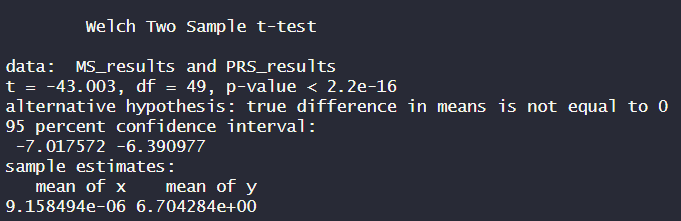
\includegraphics[width=0.9\linewidth]{img/T3.png}
     \caption{Wynik funkcji t.test.}
     \label{fig:enter-label}
 \end{figure}
Średnia wyników dla metody PRS wynosi $6.704284$, natomiast dla metody MS wynosi $9.158494*10^{-6}$. Jest to różnica 6 rzędów wielkości na korzyść metody MS. P-value wynosi $2.2*10^{-16}$, a przedział ufności nie zawiera zera. Z tego wynika że odrzucamy hipotezę zerową, czyli średnie wyników obu algorytmów nie są sobie równe.

\subsection{Wykresy funkcji Ackley’a}
\subsubsection{Pure-Random-Search}
\begin{figure}[H]
  \centering
  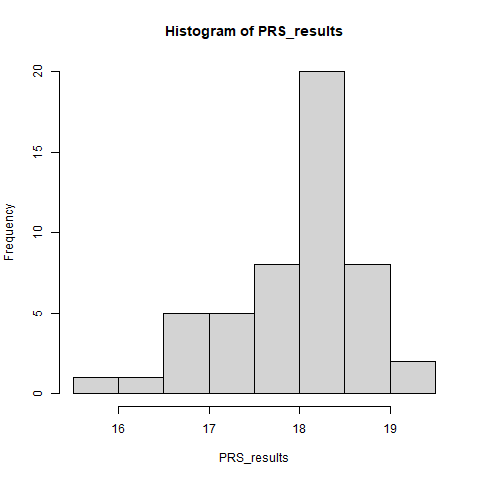
\includegraphics[width=0.7\textwidth]{img/dim10_PRS_Ackley_his.png}
  \caption{Histogram funkcji Ackley'a, metody PRS, dla 10 wymiarów.}
\end{figure}
\begin{figure}[H]
  \centering
  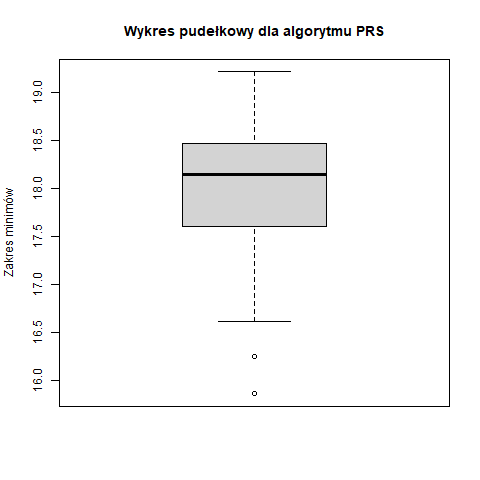
\includegraphics[width=0.56\textwidth]{img/dim10_PRS_Ackley.png}
  \caption{Wykres pudełkowy funkcji Ackley'a, metody PRS, dla 10 wymiarów.}
\end{figure}

\subsubsection{Multi-Start}
\begin{figure}[H]
  \centering
  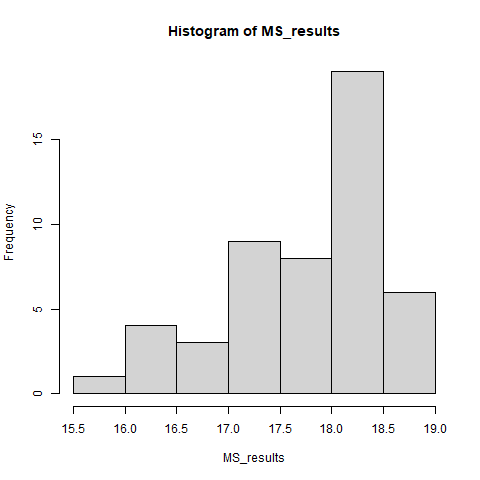
\includegraphics[width=0.56\textwidth]{img/dim10_MS_Ackley_his.png}
  \caption{Histogram funkcji Ackley'a, metody MS, dla 10 wymiarów.}
\end{figure}
\begin{figure}[H]
  \centering
  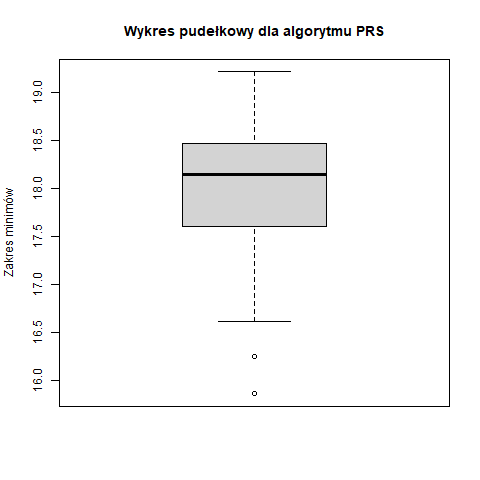
\includegraphics[width=0.7\textwidth]{img/dim10_MS_Ackley.png}
  \caption{Wykres pudełkowy funkcji Ackley'a, metody MS, dla 10 wymiarów.}
\end{figure}

\subsubsection{Obserwacje}
 \begin{figure}[H]
     \centering
     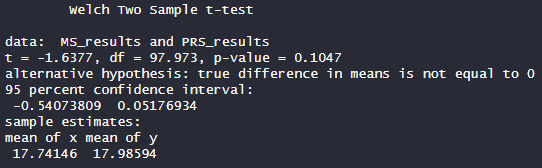
\includegraphics[width=0.9\linewidth]{img/T4.png}
     \caption{Wynik funkcji t.test.}
     \label{fig:enter-label}
 \end{figure}

Średnia wyników dla metody PRS wynosi $17.98594$, natomiast dla metody MS wynosi $17.7414$. Dokładniejsza była metoda MS. P-value wynosi $0.1047$, a przedział ufności zawiera 0. Z tego wynika że nie odrzucamy hipotezy zerowej, więc nie możemy nic powiedzieć o równości średnich.

\section{dim = 20}
\subsection{Wykresy Alpine01}
\subsubsection{Pure-Random-Search}
\begin{figure}[H]
  \centering
  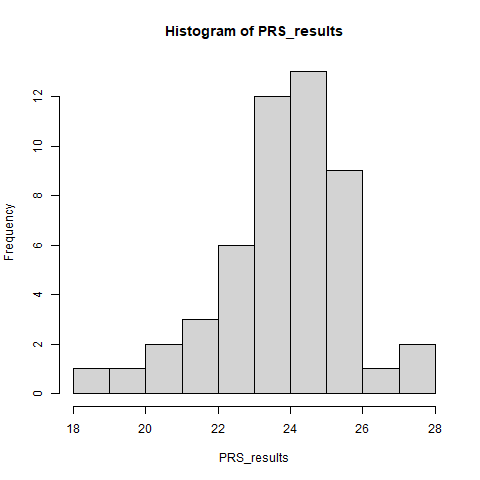
\includegraphics[width=0.7\textwidth]{img/dim20_PRS_Alpine01_his.png}
  \caption{Histogram funkcji Alpine01, metody PRS, dla 20 wymiarów.}
\end{figure}
\begin{figure}[H]
  \centering
  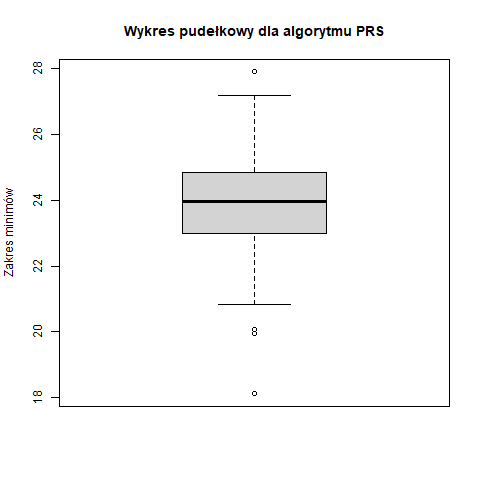
\includegraphics[width=0.56\textwidth]{img/dim20_PRS_Alpine01.png}
  \caption{Wykres pudełkowy funkcji Alpine01, metody PRS, dla 20 wymiarów.}
\end{figure}

\subsubsection{Multi-Start}
\begin{figure}[H]
  \centering
  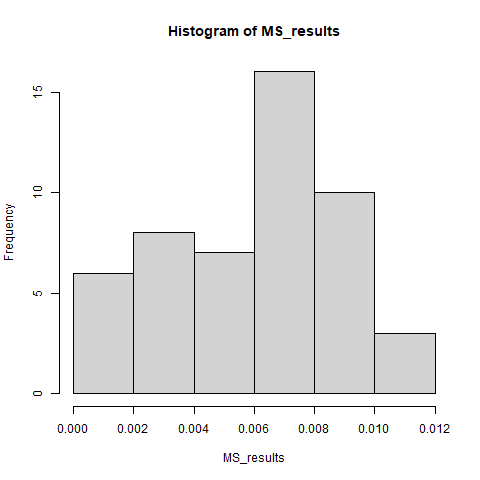
\includegraphics[width=0.56\textwidth]{img/dim20_MS_Alpine01_his.png}
  \caption{Histogram funkcji Alpine01, metody MS, dla 20 wymiarów.}
\end{figure}
\begin{figure}[H]
  \centering
  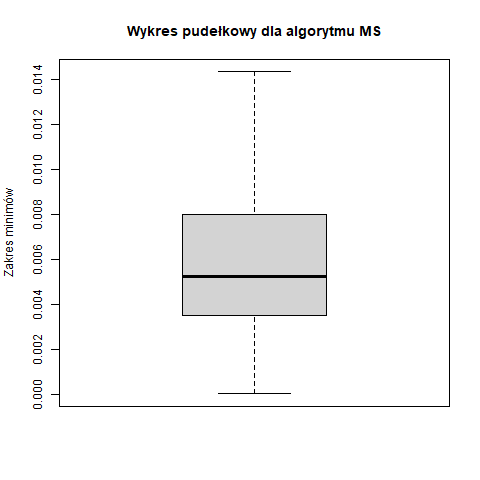
\includegraphics[width=0.7\textwidth]{img/dim20_MS_Alpine01.png}
  \caption{Wykres pudełkowy funkcji Alpine01, metody MS, dla 20 wymiarów.}
\end{figure}

\subsubsection{Obserwacje}
 \begin{figure}[H]
     \centering
     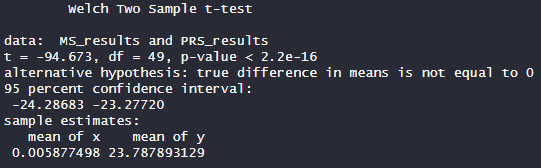
\includegraphics[width=0.9\linewidth]{img/T5.png}
     \caption{Wynik funkcji t.test.}
     \label{fig:enter-label}
 \end{figure}

Średnia wyników dla metody PRS wynosi $23.787893$, natomiast dla metody MS wynosi $5.8774*10^{-3}$. Jest to różnica 4 rzędów wielkości na korzyść metody MS. P-value wynosi $2.2^{-16}$, a przedział ufności nie zawiera 0. Z tego wynika że odrzucamy hipotezę zerową, z tego wynika że średnie nie są sobie równe.

\subsection{Wykresy funkcji Ackley’a}
\subsubsection{Pure-Random-Search}
\begin{figure}[H]
  \centering
  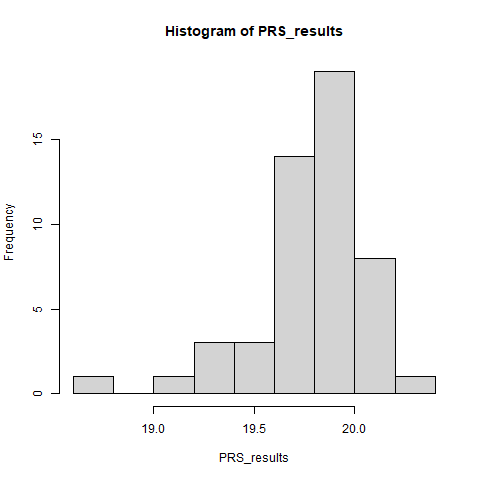
\includegraphics[width=0.7\textwidth]{img/dim20_PRS_Ackley_his.png}
  \caption{Histogram funkcji Ackley'a, metody PRS, dla 20 wymiarów.}
\end{figure}
\begin{figure}[H]
  \centering
  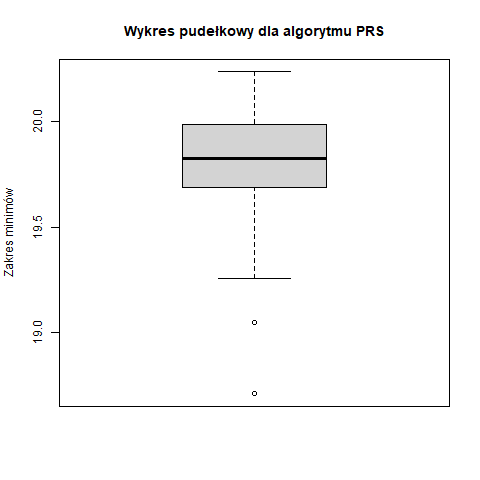
\includegraphics[width=0.56\textwidth]{img/dim20_PRS_Ackley.png}
  \caption{Wykres pudełkowy funkcji Ackley'a, metody PRS, dla 20 wymiarów.}
\end{figure}

\subsubsection{Multi-Start}
\begin{figure}[H]
  \centering
  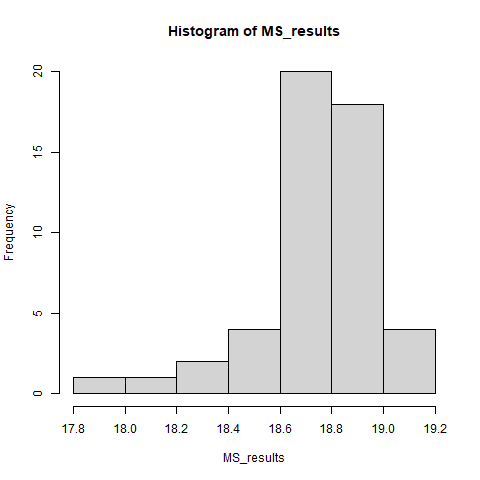
\includegraphics[width=0.56\textwidth]{img/dim20_MS_Ackley_his.png}
  \caption{Histogram funkcji Ackley'a, metody MS, dla 20 wymiarów.}
\end{figure}
\begin{figure}[H]
  \centering
  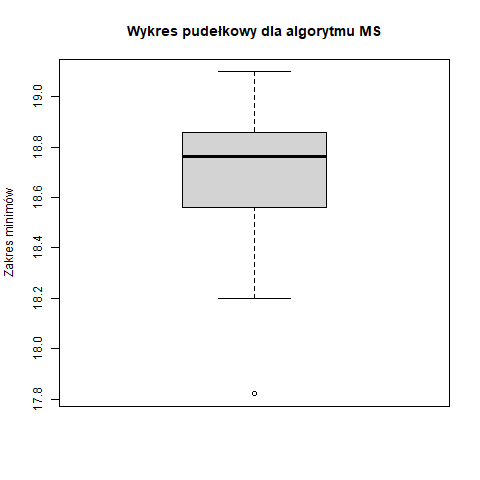
\includegraphics[width=0.7\textwidth]{img/dim20_MS_Ackley.png}
  \caption{Wykres pudełkowy funkcji Ackley'a, metody MS, dla 20 wymiarów.}
\end{figure}

\subsubsection{Obserwacje}
 \begin{figure}[H]
     \centering
     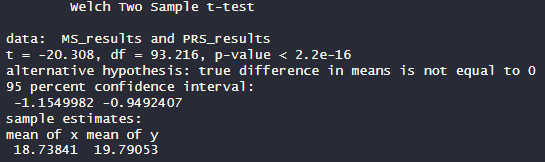
\includegraphics[width=0.9\linewidth]{img/T6.png}
     \caption{Wynik funkcji t.test.}
     \label{fig:enter-label}
 \end{figure}

Średnia wyników dla metody PRS wynosi $19.7905$, natomiast dla metody MS wynosi $18.7384$. Metoda MS jest nieznacznie dokładniejsza. P-value wynosi $2.2^{-16}$, a przedział ufności nie zawiera 0. Z tego wynika że odrzucamy hipotezę zerową, z tego wynika że średnie nie są sobie równe.

\newpage
\part{Podsumowanie}
\section{Podsumowanie}
Na podstawie przeprowadzonych porównań można zauważyc że metoda MS jest skuteczniejszym algorytmem znajdowania minimum funkcji. Zazwyczaj wyniki były zauważalnie lepsze dla metody MS. Dzieje się tak, ponieważ metoda PRS opiera się na losowym wyborze punktów pomiarowych, w odróżnieniu od metody MS która wykorzystuje informacje o gradiencie funkcji do wyznaczenia kierunku optymalizacji.
\par
Wraz ze wzrostem liczby wymiarów wyniki obu metod pogarszają się. Przyczyną tego stanu rzeczy jest wzrastające skomplikowanie problemu przy stałej liczbie losowanych punktów.
\newline\par
Metoda PRS ze względu na swoją losowość nie zależy tak bardzo od charakterystyki testowanej funkcji. W odróżnieniu od metody MS, która jest wrażliwa na ukształtowanie gradientu, co jest szczególnie zauważalne przy badaniu funkcji Ackley'a dla której obie metody  dawały zbliżone wyniki. 
\par
Analiza funkcji Alpine01 wykazała, że metoda MS była zdecydowanie skuteczniejsza ze względu na optymalizację wyboru minimum na podstawie gradientu funkcji.
\newline\par
W pięciu na sześć porównań z analizy istotności statystycznej różnicy między średnim wynikiem obu algorytmów, opartej na 95-procentowym przedziale ufności odrzuciliśmy hipoteze zerową zakładającą równość obu średnich na rzecz hipotezy alternatywnej zakładającej to że średnie są od siebie różnie.
\par
W jednym przypadku hipoteza zerowa nie została odrzucona, wyniki obu algorytmów w tamtym przypadku mocno odbiegają od realnego minimum lokalnego i prawdopodobnie przypadkowo są do siebie bardzo zbliżone co jest przyczyną tego że nie można jednoznacznie określić czy te średnie różnią się od siebie przy zadanym przedziale ufności.





\newpage
\section{Bibliografia}
Źródła i inspiracje wykorzystane przy tworzeniu projektu:
\begin{itemize}
  \item Wykłady z Rachunku prawdopodobieństwa i statystyki, prowadzone przez dr hab. Macieja Smółkę, na 3 semestrze Informatyki AGH WI.
  \item \url{https://www.agh.edu.pl/o-agh/multimedia/znak-graficzny-agh/}
  \item \url{http://infinity77.net/global_optimization/test_functions_nd_A.html}
  \item
  \url{https://pogotowiestatystyczne.pl/aploud/2023/04/2023-02-Test-t-Studenta-dla-prob-niezaleznych.pdf}
\end{itemize}

\end{document}